\documentclass{beamer}

\usepackage[utf8]{inputenc}
\usepackage{float}
\usepackage{graphicx}
\usepackage{amsmath}
\usepackage[turkish]{babel}

\author{Deniz Koluaçık}
\title{Make}
\subtitle{Or How I Learned To Stop Worrying And Love The Compilation Process}
\setbeamertemplate{frametitle}{\vspace*{2mm}\begin{center} \insertframetitle\end{center}}

\begin{document}
    
%\usebackgroundtemplate{
\includegraphics[scale=2]{images/full_base2.png}}
{
\usebackgroundtemplate{
\includegraphics{images/full_base2.png}}
\begin{frame}
    \titlepage{}
    
\end{frame}
}

{
\usebackgroundtemplate{
\includegraphics{images/gnu_make.png}}
\begin{frame}
    \frametitle{İçindekiler}
    \
    \tableofcontents
    
\end{frame}
}

\section{Neden Make? (Derleme Kabusu)}
{
\usebackgroundtemplate{
\includegraphics{images/soru1.png}}
\begin{frame}
    \frametitle{Neden Make?}
    
\end{frame}
}

{
\usebackgroundtemplate{
\includegraphics{images/program.png}}
\begin{frame}
   \footnote{Aslında dosyaların derlenebilmesi için böyle bir gereklilik ağacı mevcut değil. Yani diğer .c dosyalarının derleme esnasında bir arada olması gerekmiyor, bu gereklilik linkleme anında açığa çıkıyor. Buradaki grafik programın parçaları arasındaki mantıksal gereklilik ağacı.}

    
\end{frame}
}
{
%\usebackgroundtemplate{
\includegraphics[scale=1]{images/compile1.png}}
\begin{frame}
    \frametitle{Naif Yöntem}
    \texttt{gcc -o main main.c lib2.c lib21.c lib22.c lib1.c}\\
    \vspace{4mm}
    Sıkıntılar:
    \begin{itemize}
        \item Ufak değişikliklerde bütün dosyalar tekrar derlenir, zaman ve enerji\ldots
        \item Dosya sayısı arttıkça karmaşıklaşır.
    \end{itemize}

    
\end{frame}
}

\begin{frame}
    \frametitle{Başka Bir Naif Yöntem}
    \texttt{gcc -c -o lib21.o lib21.c\\
    gcc -c -o lib22.o lib22.c\\
    gcc -c -o lib2.o lib2.c\\
    gcc -c -o lib1.o lib1.c\\
    gcc -c -o main.o main.c\\
    gcc -o main main.o lib1.o lib21.o lib22.o lib2.o}\\
    \vspace{4mm}
    Sıkıntılar:
    \begin{itemize}
        \item Kullanıcı hangi komutların gerekli olduğunu düşünmelidir\footnote{Asıl sıkıntı header dosyalarında bir değişiklik yapıldığında başlıyor.}.
            \item Fazlasıyla karmaşık.
    \end{itemize}
\end{frame}
{
\usebackgroundtemplate{
\includegraphics{images/soru2.png}}
\begin{frame}

    
\end{frame}
}
{
\usebackgroundtemplate{
\includegraphics{images/blue_screen.png}}
\begin{frame}
    \frametitle{Linux 5.5 70,000'den Fazla Dosyadan Oluşuyor}
    Soru: Derleme işlemini daha\\ kolay yapmanın bir yolu var mı?
    
\end{frame}
}

{
\usebackgroundtemplate{
\includegraphics{images/blue_screen.png}}
\begin{frame}
    {Make!}
    1976 Stuart Feldman (Bell Labs)\\
    1988 GNU Project
\end{frame}
}

\section{MAKE100: Make Nasıl Çalışır?}
{
\usebackgroundtemplate{
\includegraphics{images/100.png}}
\begin{frame}
    {MAKE100: Make Nasıl Çalışır?}
    \begin{itemize}
        \item{Çalışma Mantığı}
        \item{Temel Syntax}
    \end{itemize}
\end{frame}
}

\subsection{Mantık}
\begin{frame}
    {Make Dosyasının İçeriği}

    \texttt{target: prerequisites\\ \hspace{10mm}recipe }\\\vspace{3mm}
    \texttt{target: prerequisites\\ \hspace{10mm}recipe }\\\vspace{3mm}
    \texttt{target: prerequisites\\ \hspace{10mm}recipe }\\\vspace{3mm}

    (Her biri bir kural.)

\end{frame}

\begin{frame}
    {Örnek}

    \texttt{main: main.o lib1.o \\
    \hspace{10mm}	gcc -o main main.o lib1.o \\\vspace{3mm}
main.o: main.c lib1.h\\
	\hspace{10mm}	gcc -c -o main.o main.c\\\vspace{3mm}
lib1.o: lib1.h lib1.c\\
    \hspace{10mm}	gcc -c -o lib1.o lib1.c\\}
    
\end{frame}

\subsubsection{Target, Recipe, Prerequisite\ldots}
{
\usebackgroundtemplate{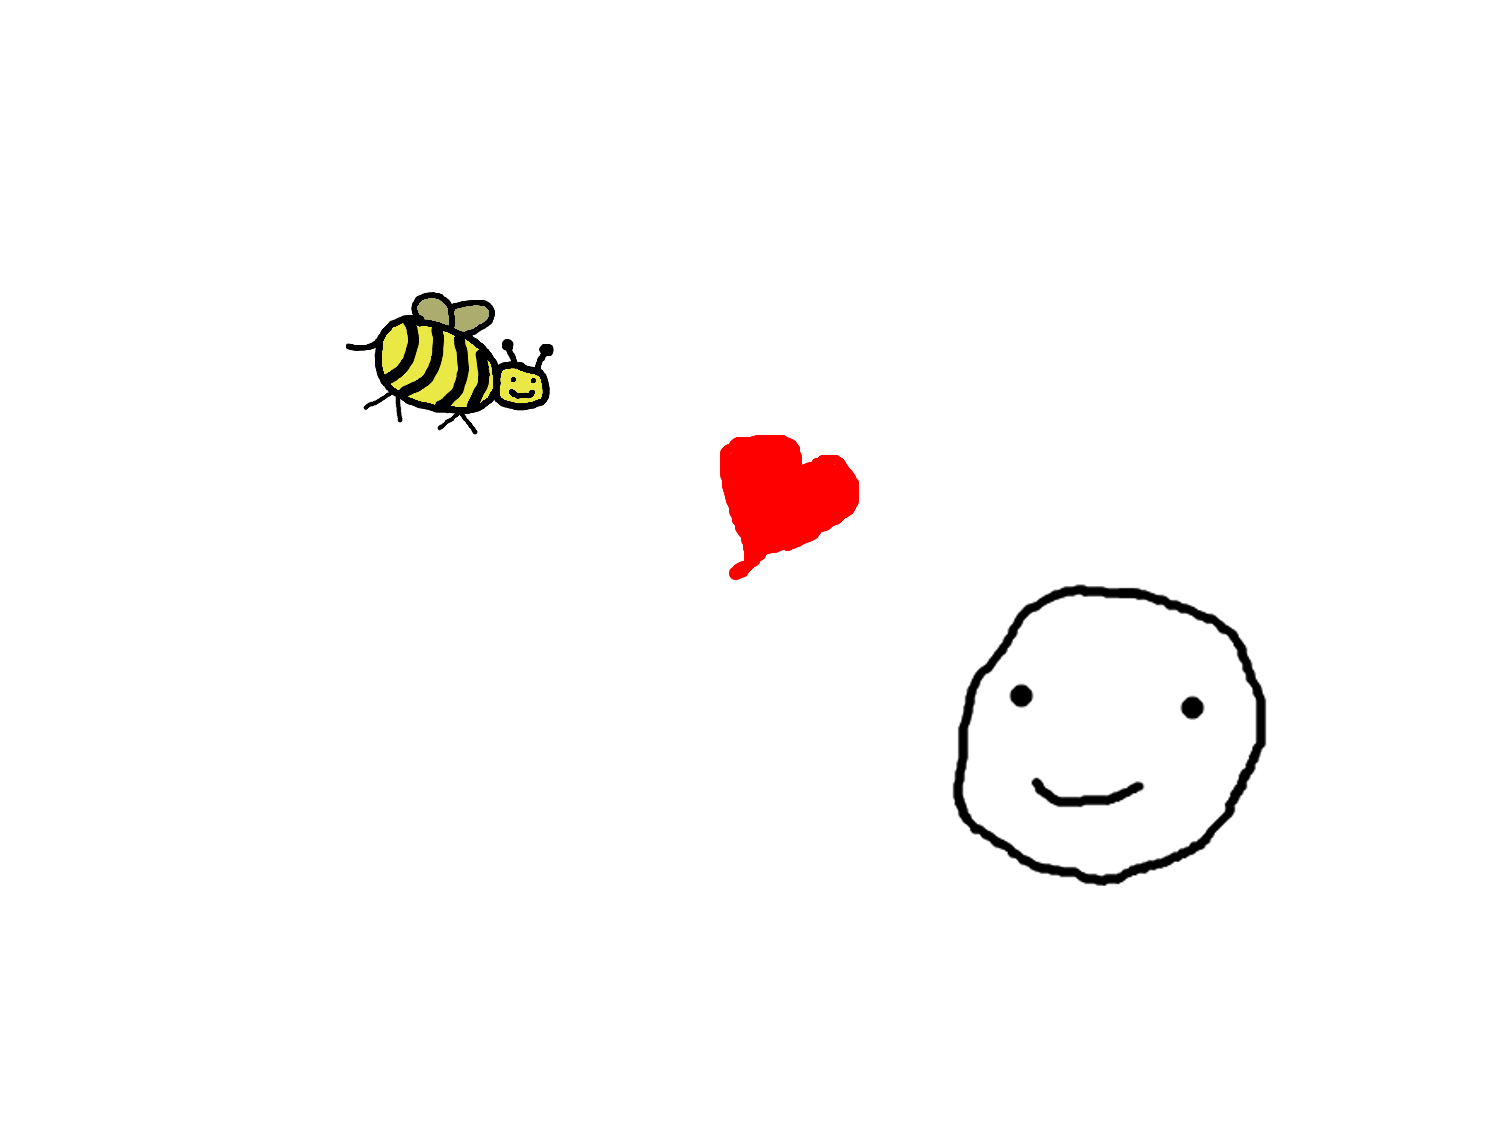
\includegraphics{images/kalp.png}}
\begin{frame}
{Target, Recipe, Prerequisite}
\end{frame}
}

\subsubsection{İşleyiş ve Recursion}
\begin{frame}
    {Target'ı (Yeniden) Oluşturmalı Mı?}
    Herhangi bir target için:
    \begin{itemize}
        \item Prerequisite bir Target'sa onu oluşturmalı mı?\footnote{Recursion!}
        \item Target var mı, varsa güncel mi? (son değiştirilme)
            \begin{itemize}
                \item Hayır: \textbf{Target'ı oluştur.}
                \item Evet: \textbf{Target güncel.}

            \end{itemize}
    \end{itemize}
        
\end{frame}

\begin{frame}

    \texttt{main: main.o lib1.o \\
    \hspace{10mm}	gcc -o main main.o lib1.o \\\vspace{3mm}
main.o: main.c lib1.h\\
	\hspace{10mm}	gcc -c -o main.o main.c\\\vspace{3mm}
lib1.o: lib1.h lib1.c\\
    \hspace{10mm}	gcc -c -o lib1.o lib1.c\\}
    
\end{frame}

\subsection{Temel Syntax}
\begin{frame}
    {Syntax}
    \texttt{main: main.o lib1.o \\
    \hspace{10mm}	gcc -o main main.o lib1.o}
\end{frame}
\subsubsection{Recipes}
\begin{frame}
    \texttt{main: main.o lib1.o \\
    \hspace{10mm}	gcc -o main main.o lib1.o\\
    \hspace{10mm}   echo "Iyi günler!"}
\end{frame}
\subsubsection{Variables, Substitutions}
\begin{frame}
    {Variables}
    \texttt{%
        VAR = main\\
        \$(VAR): main.o lib1.o\ldots}\\
        \vspace{5mm}
        \pause{}
    \texttt{%
        gcc -Wall -ansi -pedantic-errors -g -O0 -o main main.o lib1.o}\\
        \vspace{2mm}
        yerine\ldots\\
        \vspace{2mm}
    \texttt{%
        FLAGS = -Wall -ansi -pedantic-errors -g -O0\\
        gcc \$(FLAGS) -o main main.o lib1.o}
        
\end{frame}

\begin{frame}
    \texttt{%
        OBJECTS = main.o lib1.o lib21.o lib22.o lib2.o\\
        main: \$(OBJECTS)\\
        \hspace{10mm}   gcc -o main \$(OBJECTS)}
\end{frame}

\begin{frame}
    {Wildcards}
    \texttt{*.o}: sonu ``\texttt{.o}'' ile biten bütün dosyalar.\\
    \vspace{5mm}
    \texttt{%
        clean:\\
        \hspace{10mm}   rm main\\
        \hspace{10mm}   rm *.o\\}


    
\end{frame}
{
\usebackgroundtemplate{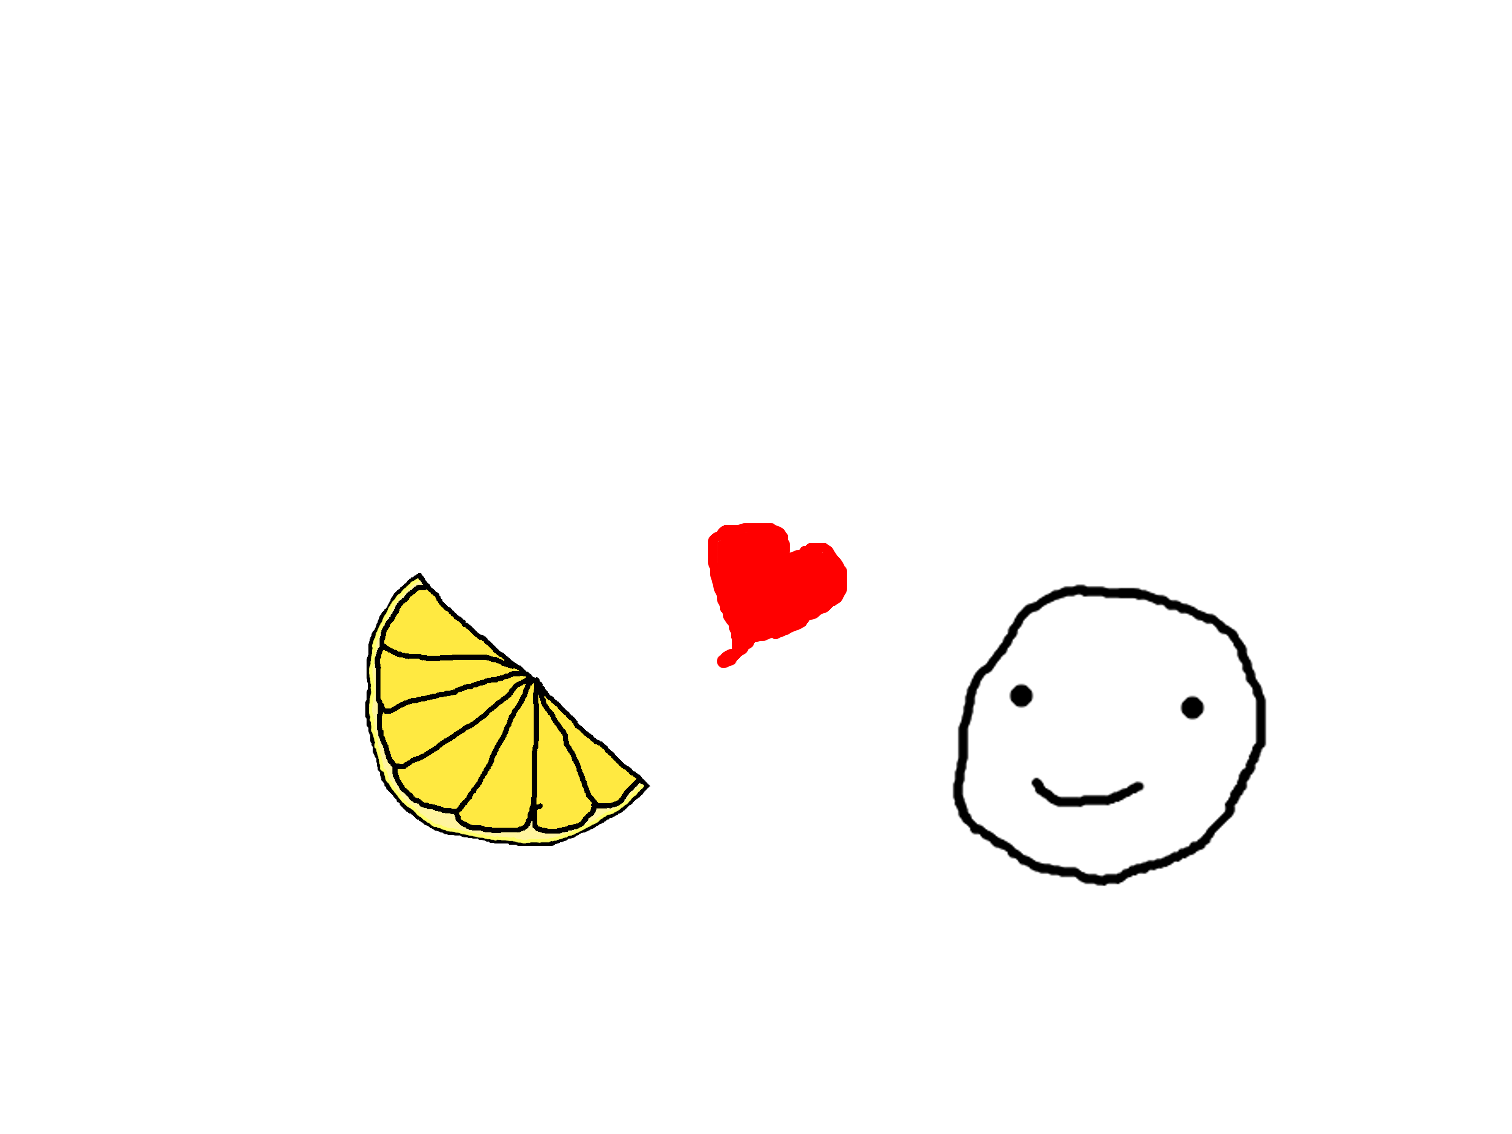
\includegraphics{images/li.png}}
\begin{frame}
    {Artık Kendi Makefile'ımızı Yazabiliriz!}
\end{frame}
}


\section{MAKE200: Güçlü Özellikler}
{
\usebackgroundtemplate{
\includegraphics{images/buff_base.png}}
\begin{frame}
    {MAKE200: Güçlü Özellikler!}
\end{frame}
}

\subsection{Errors, Phony Targets}
\begin{frame}
    {Ignoring errors}

\texttt{%
        clean:\\
        \hspace{10mm}   rm main\\
        \hspace{10mm}   rm *.o\\}

        \vspace{5mm}

        Peki ya ``main'' dosyası o an yoksa?

\end{frame}

\begin{frame}
    {Ignoring Errors}

\texttt{%
        clean:\\
        \hspace{10mm}   -rm main\\
        \hspace{10mm}   -rm *.o\\}

        \vspace{5mm}

        Başına ``-'' konan satırlarda karşılaşılan hatalar tarifi durdurmaz.

\end{frame}

\begin{frame}
    {Phony Targets}

\texttt{%
        clean:\\
        \hspace{10mm}   -rm main\\
        \hspace{10mm}   -rm *.o\\}

        \vspace{5mm}

        Peki ya dizinde ``clean'' isimli bir dosya varsa?\\
        \vspace{3mm}
        \texttt{Make: `clean' is up to date.}

\end{frame}

\begin{frame}
    {Phony Targets}

\texttt{%
    .PHONY: clean\footnote{.PHONY sadece özel adı olan bir kuraldır.}\\
        clean:\\
        \hspace{10mm}   -rm main\\
        \hspace{10mm}   -rm *.o\\}

        \vspace{5mm}
        Dizinde `clean' isimli bir dosya olsa bile bu kural düzgün çalışır.

        \vspace{3mm}

\end{frame}

\begin{frame}
    {Recipe Echoing}

\texttt{%
        .PHONY: clean\\
        clean:\\
        \hspace{10mm}   -@rm main\\
        \hspace{10mm}   -@rm *.o\\}

        \vspace{5mm}
Make tarifte yer alan bütün komutları yazdırır.\\
    Bunun önüne geçmek için satırların önüne `@' konulabilir.\\         \vspace{3mm}
    Özellikle \texttt{echo} komutlarının başına yazmak çok iyi bir fikir.

\end{frame}


\subsection{Implicit Variables and Rules}
\begin{frame}
    {Implicit Variables}
    \$(CC): C Compiler, cc (cc $\rightarrow$ gcc, symlink\footnote{ls -l /usr/bin/cc}) \\
    \$(CXX): C++ Compiler, g++ \\
    \$(CFLAGS): C flags, empty string \\
    \$(CXXFLAGS): C++ flags, empty string \\
    \vspace{3mm} 
    \$(CPPFLAGS): C Preprocessor flags, empty string.

\end{frame}

\begin{frame}
    {Implicit Rules}

    make yaygın bazı kuralları otomatik olarak oluşturur.\\
    \vspace{3mm}

    \texttt{%
        foo.o: foo.c \\
        \hspace{10mm}   \$(CC) \$(CPPFLAGS) \$(CFLAGS) -c -o foo.o foo.c\\
        }
        \vspace{3mm}
        Benzeri cpp için de mevcut. (CXX, CXXFLAGS)\\
\end{frame}

\begin{frame}
    \begin{itemize}
    \item Implicit rule'ların çalışması için dosyada o Target ve Prerequisite'lerin varlığından söz etmeye gerek yoktur.\\
        \texttt{make lib22.o}
    \item Yine de istersek bir bir Target'a elle Prerequisite belirleyerek Implicit rule'a katkıda bulunabiliriz.\\
        \texttt{lib1.o: lib1.c lib.h}
    \item Implicit rule'lar zincirleme çalışabilir. Bir prerequisite'in implicit bir tarifi olabilir.
        
    \end{itemize}
\end{frame}

\begin{frame}
    {Implicit Linking Rule}
    .c(pp) dosyalarını derlemek için olduğu gibi .o dosyalarını linklemek için de bir Implicit rule mevcut.\\
    \vspace{5mm}

    \texttt{%
        n: n.o\\
        \hspace{10mm} \$(CC) \$(LDFLAGS) n.o \$(LOADLIBES) \$(LDLIBS)\\
        }

        Birden fazla .o dosyasını linklemek için Target ve Prerequisite belirtmeliyiz.\\
    \vspace{5mm}
    \texttt{%
        main: main.o lib1.o lib2.o lib21.o lib22.o\\
        }
        
\end{frame}

\subsection{Pattern Rules, Automatic Variables}
\begin{frame}
    {Pattern Rules}
    \texttt{%
        lib1.o: lib1.h lib1.c\\
        lib2.o: lib2.h lib2.c\\
        lib21.o: lib21.h lib21.c\\
        lib22.o: lib22.h lib22.c\\
        }
        \vspace{5mm}
        Genelleştirilebilir.

\end{frame}

\begin{frame}
    \texttt{%
        \%.o: \%.c \%.h\\
        }
        \vspace{5mm}
        \%, make xxx.o formatında girilen herhangi bir komutta xxx'in değerini alır.\\
        \%, herhangi bir prefix ve suffixle tanımlanabilir. (of\%off gibi)\\
        \%, empty string olamaz.\\
        \%'nun değerini aldığı string'e \textit{stem} denir.


\end{frame}

\begin{frame}
    {Automatic Variables}
    Bir kuralın çalıştırılması anında değer alan değişkenlerdir.\\
    Pattern rule'larda çok faydalıdır.\\
    \vspace{5mm}
    \$@: Target'ın ismi.
        \vspace{3mm}

    \texttt{%
        he\%he:\\
        \hspace{10mm} @echo \$@
        }
        \vspace{5mm} (make hehehe, stdout'a hehehe yazdırır.)
    
\end{frame}

\begin{frame}
    {Başlıca Automatic Variable'lar}
    Çok sayıda tanımlı automatic variable var. Başlıcaları şunlar:
    \begin{itemize}
            \item \$@ : Target adı  \\
            \item \$$<$ : İlk prerequisite \\
            \item \$\^{} : Bütün preprequisite'ler \\
            \item \$\% : Stem  \\
        
    \end{itemize}
\vspace{5mm} 
    \texttt{%
        he\%he:\\
        \hspace{10mm} @echo \$*
        }
        \vspace{5mm} (make hehehe, stdout'a he yazdırır.)
    
\end{frame}

\begin{frame}
    {Gerçekçi Bir Örnek}
    \texttt{%
        \%.o: \%.c \%.h\\
        \hspace{10mm} @echo "making \$@!" \\ 
        \hspace{10mm} \$(CC) \$(CPPFLAGS) \$(CFLAGS) -c -o \$@  \$<\\ 
        }

    
\end{frame}

\subsection{Static Pattern Rules}
\begin{frame}
    Sorun: Implicit rule'ların dışında bir genel kural istiyorum, ama bunu pattern matching kadar genel bir şekilde değil, birkaç dosya için yapmak istiyorum.
\end{frame}

\begin{frame}
    {Static Pattern Rules!}
    
    Pattern rules, ama belli hedefler için.\\
        \vspace{5mm}

    \texttt{%
        Targets: Pattern: Prerequisites\\
        \hspace{10mm} Recipes\ldots\\
        }
    
\end{frame}

\begin{frame}
    \texttt{%
        lib1.o lib2.o lib21.o lib22.o : \%.o: \%.c \%.h\\
        \hspace{10mm} \$(CC) \$(CFLAGS) -c -o \$@ \$<\\
    }

    \vspace{5mm}
    Targets kısmı için variable kullanabiliriz.

    
\end{frame}

\begin{frame}
    \texttt{%
        LIBOBJ = lib1.o lib2.o lib21.o lib22.o\\
        \$(LIBOBJ): \%.o: \%.c \%.h\\
        \hspace{10mm} \$(CC) \$(CFLAGS) -c -o \$@ \$<\\
    }

    \vspace{5mm}

    
\end{frame}
{
\usebackgroundtemplate{
\includegraphics{images/soru1.png}}
\begin{frame}
    
\end{frame}
}

\begin{frame}
    {Şimdi Nereye?}

    \texttt{%
        \$ info make} \\
        

    
\end{frame}

{
\usebackgroundtemplate{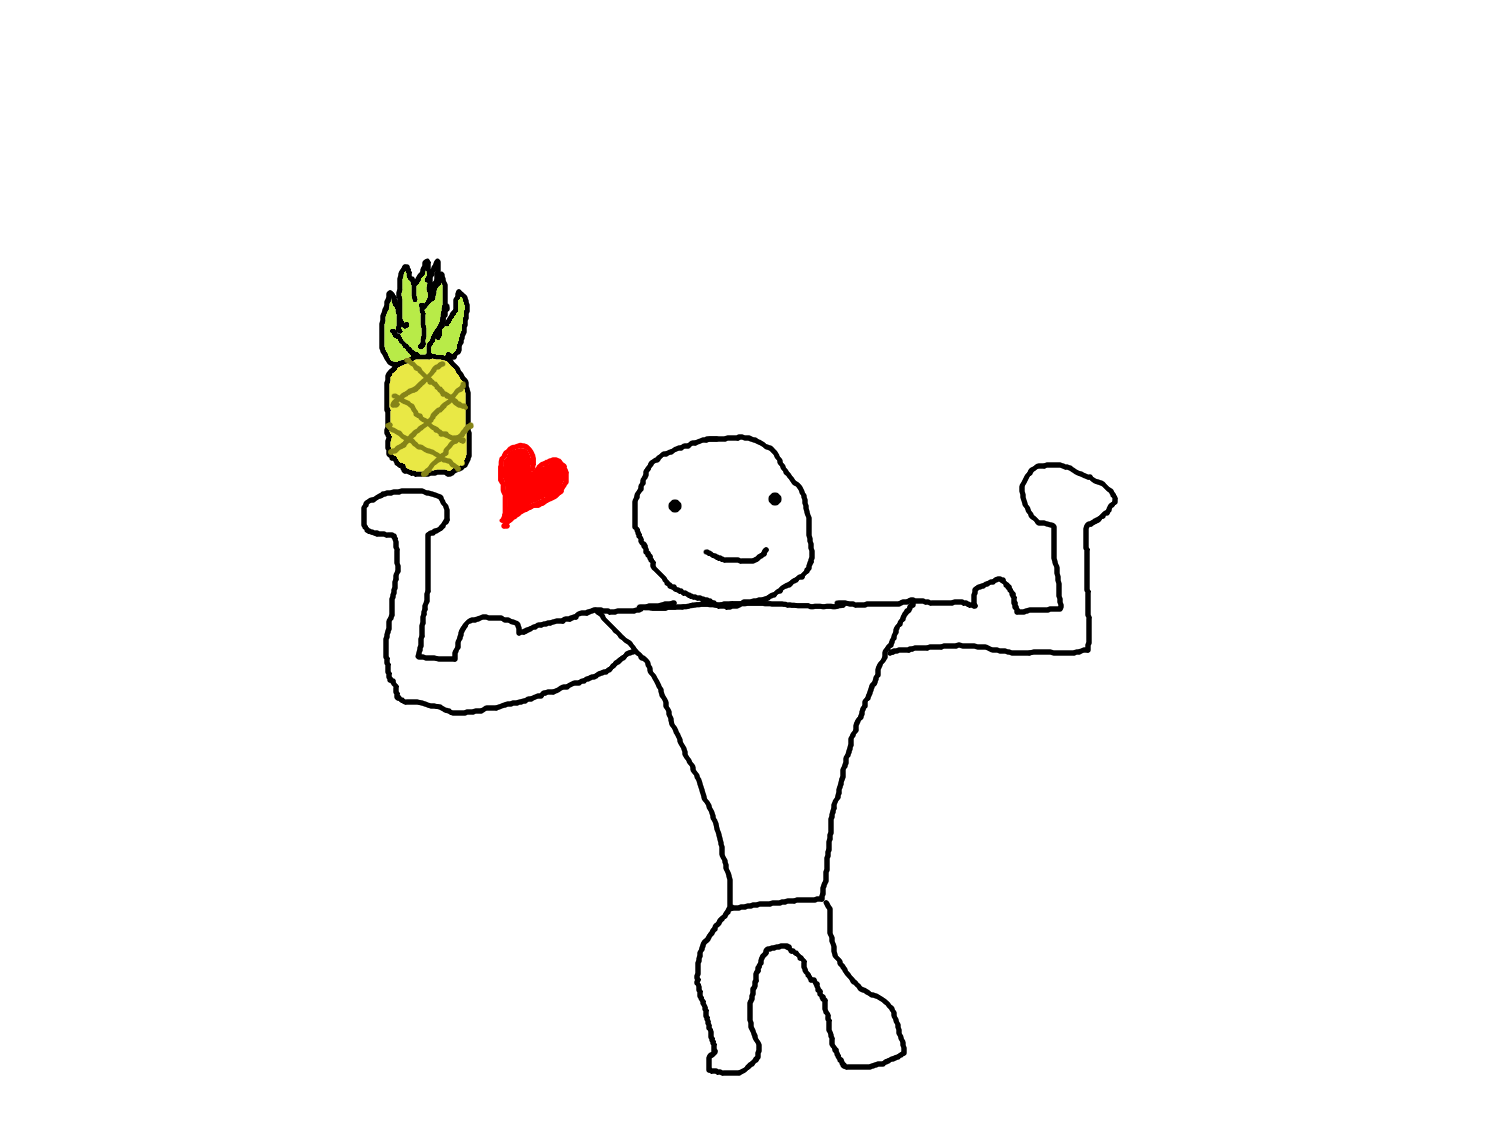
\includegraphics{images/buff_pineapple.png}}
\begin{frame}
    {Dinlediğiniz İçin Teşekkürler}

    
\end{frame}
}


\end{document}
